\appendix

\section{Canonicalization Scheme}
\label{app:token-grammar}

We demarcate memory operands (consisting of a base address, and an optional offset and displacement) by surrounding them with \texttt{<M>} and \texttt{</M>} delimiter tokens.


The following is the full grammar for the token strings, as described in Section~\ref{sec:canonicalization}.
\begin{align*}
  \textit{<block>} &::= \textit{<instr>}+\\
  \textit{<instr>} &::= \textit{opcode}\ \texttt{<S>}\ \textit{<opnd>}\hspace{-.2em}*\ \texttt{<D>}\ \textit{<opnd>}\hspace{-.2em}*\ \texttt{<E>} \\
  \textit{<opnd>} &::= \textit{register} \; | \; \texttt{<M>}\ \textit{register}\hspace{-.2em}+ \texttt{</M>} \; | \; \texttt{CONST}
\end{align*}

\section{Training Hyperparameters}
\label{app:hyperparams}

Here we present the hyperparameters for the model as described in Section~\ref{sec:model}.
All vectors, including the embedding width, hidden, and output states have width 256.
We train our models using asynchronous SGD, with a batch size of $4$, and $6$ parallel trainers.
The initial learning rate is $0.1$, and after the first $2$ epochs, it decreases by a geometric factor of $1.2$ every epoch.
We use the default PyTorch formulation for momentum (i.e. not Nesterov momentum) with $\beta=0.9$.
Each parallel trainer samples without replacement from the dataset until all training data is exhausted.
If a trainer hits a \texttt{NaN} gradient, that trainer is halted for the remainder of the epoch, and the elements in that trainer's batch are dropped for the epoch.
At the beginning of the next epoch, all trainers are restarted.
Training halts once all trainers are halted and an epoch cannot be completed.

\section{Heatmaps of Different Prediction Methods}
\label{app:heatmaps}

Figure~\ref{fig:heatmaps} shows all prediction heatmaps for \tool{}, llvm-mca and IACA under the Intel Ivy Bridge, Haswell and Skylake microarchitectures.
Note that the latest IACA version does not support Ivy Bridge and hence its prediction heatmap is not available.

\begin{figure*}
	\centering
	\subfloat[][\tool{}]{
		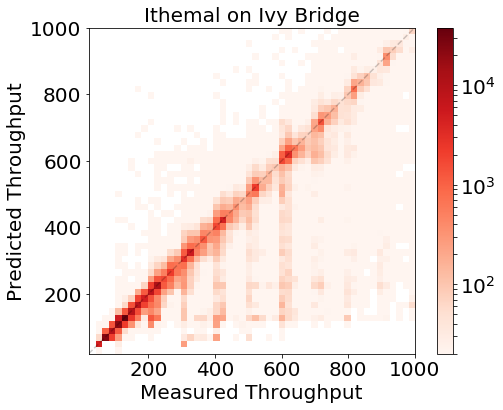
\includegraphics[width=0.33\textwidth]{figures/heatmap_ithemal_ivybridge.png}
	}
	\subfloat[][llvm-mca]{
		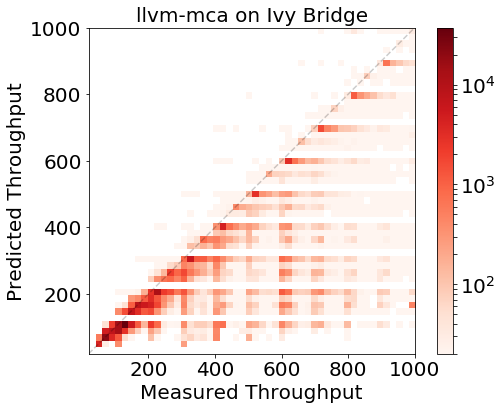
\includegraphics[width=0.33\textwidth]{figures/heatmap_llvm_ivybridge.png}
	}\\
	\subfloat[][\tool{}]{
		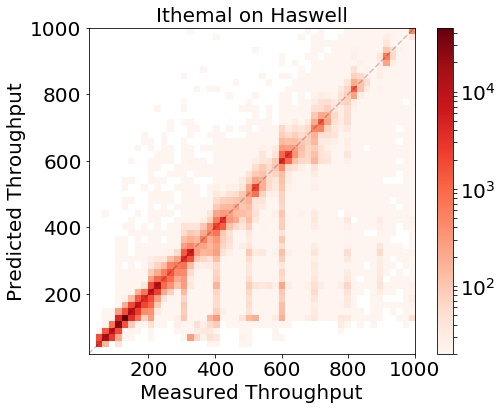
\includegraphics[width=0.33\textwidth]{figures/heatmap_ithemal_haswell.png}
	}
        \subfloat[][llvm-mca]{
		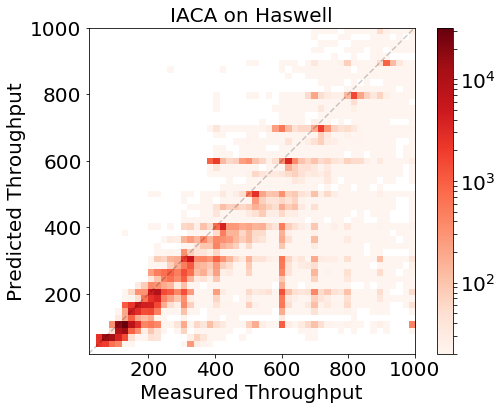
\includegraphics[width=0.33\textwidth]{figures/heatmap_iaca_haswell.png}
	}
        \subfloat[][IACA]{
		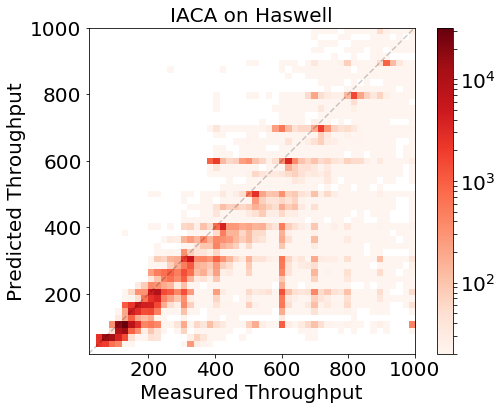
\includegraphics[width=0.33\textwidth]{figures/heatmap_iaca_haswell.png}
	}\\

	\subfloat[][\tool{}]{
		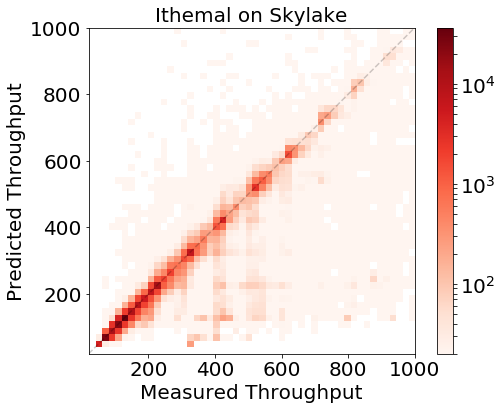
\includegraphics[width=0.33\textwidth]{figures/heatmap_ithemal_skylake.png}
	}
        \subfloat[][llvm-mca]{
		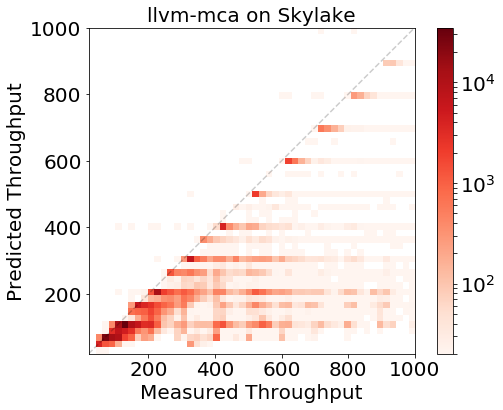
\includegraphics[width=0.33\textwidth]{figures/heatmap_llvm_skylake.png}
	}
        \subfloat[][IACA]{
		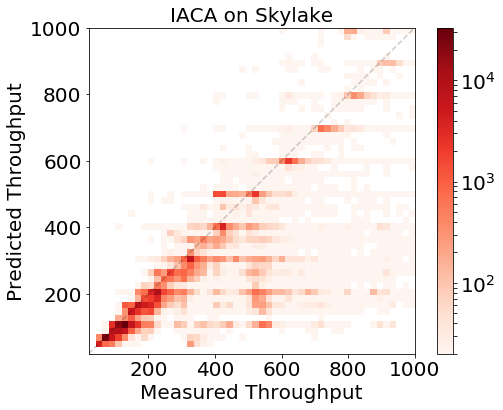
\includegraphics[width=0.33\textwidth]{figures/heatmap_iaca_skylake.png}
	}



	\caption{Heatmaps for measured and predicted throughput values under different models for basic blocks with measured throughput values less than 1000 cycles for the Intel Ivy Bridge, Haswell and Skylake microarchitectures}
	\label{fig:heatmaps}
\end{figure*}


\section{Prediction Errors for Throughput Ranges}
\label{app:error}

Figure~\ref{fig:errorall} shows how the average error changes between various throughput ranges for each prediction method under different microarchitectures for basic blocks with throughput values under 1000 cycles.
Throughput values are broken up in to bins of length and width 20 cycles on each axis.
It also shows the throughput distribution of the basic blocks, and the average error across different measured throughput ranges.
\tool{} consistently predicts throughput values with lower average errors compared to llvm-mca and IACA.
Overall, \tool{} is more robust in its prediction across all throughput ranges compared to llvm-mca and IACA which show higher fluctuations.

\begin{figure*}
	\centering
	\subfloat[][Ivy Bridge - error curve]{
		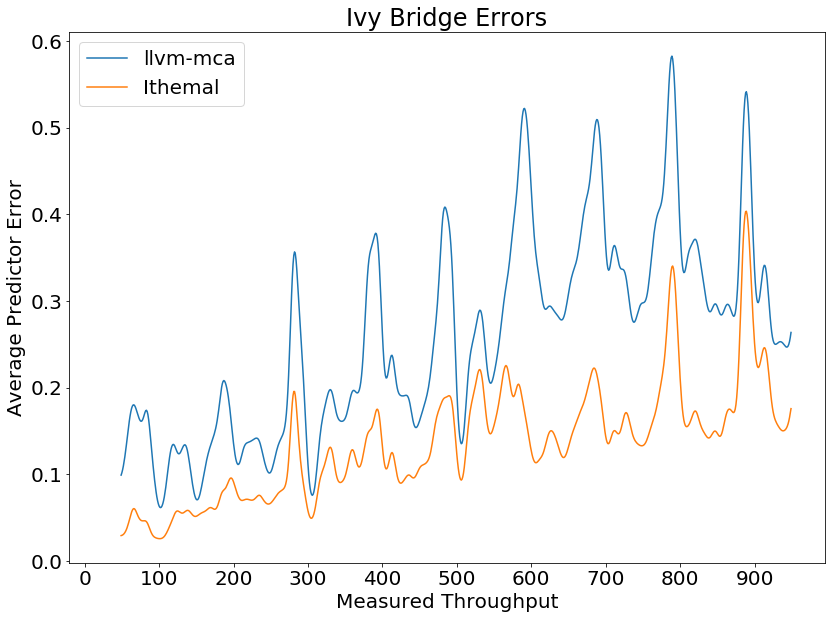
\includegraphics[width=0.33\textwidth]{figures/txput_error_ivybridge.png}
	}
        \subfloat[][Ivy Bridge - throughput distribution]{
		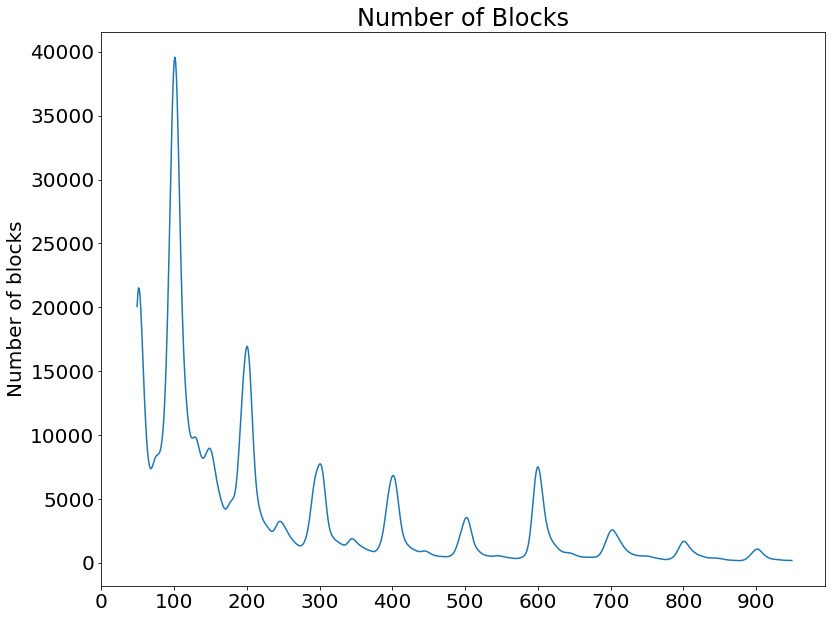
\includegraphics[width=0.33\textwidth]{figures/txput_count_ivybridge.png}
	}
        \subfloat[][Ivy Bridge - best predictor percentage]{
		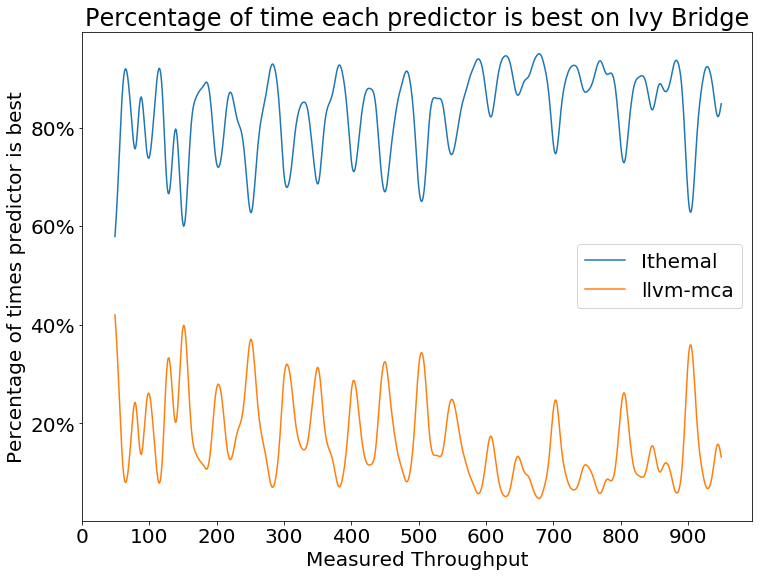
\includegraphics[width=0.33\textwidth]{figures/txput_win_ivybridge.png}
	}\\
	\subfloat[][Haswell - error curve]{
		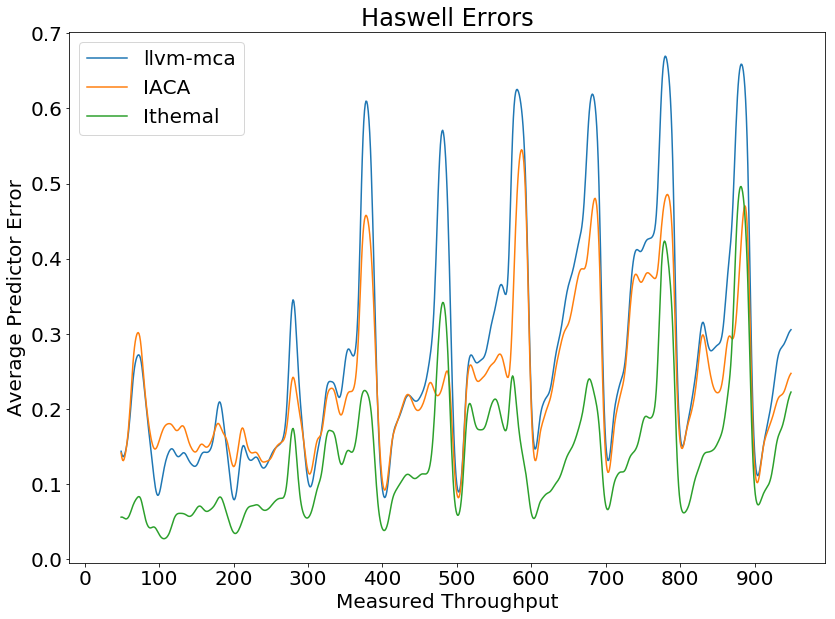
\includegraphics[width=0.33\textwidth]{figures/txput_error_haswell.png}
	}
        \subfloat[][Haswell - throughput distribution]{
		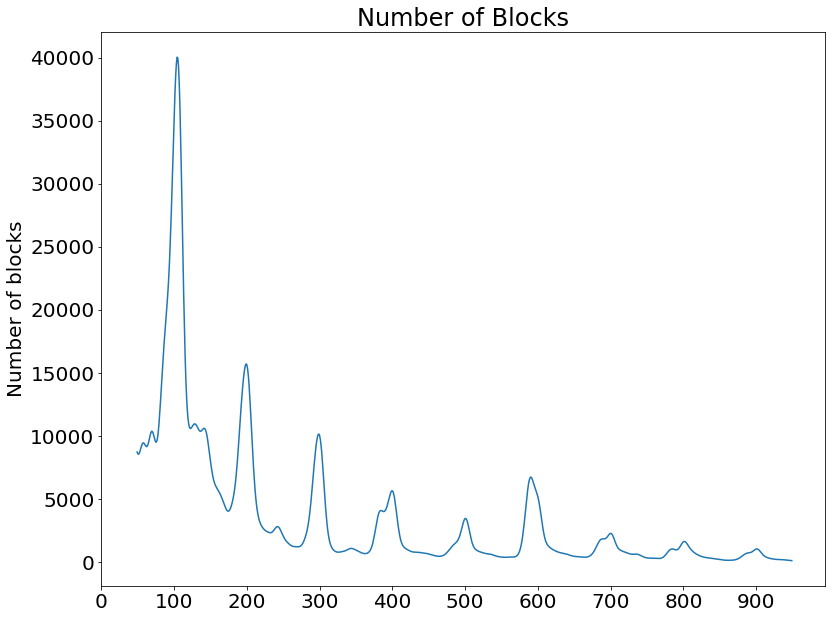
\includegraphics[width=0.33\textwidth]{figures/txput_count_haswell.png}
	}
        \subfloat[][Haswell - best predictor percentage]{
		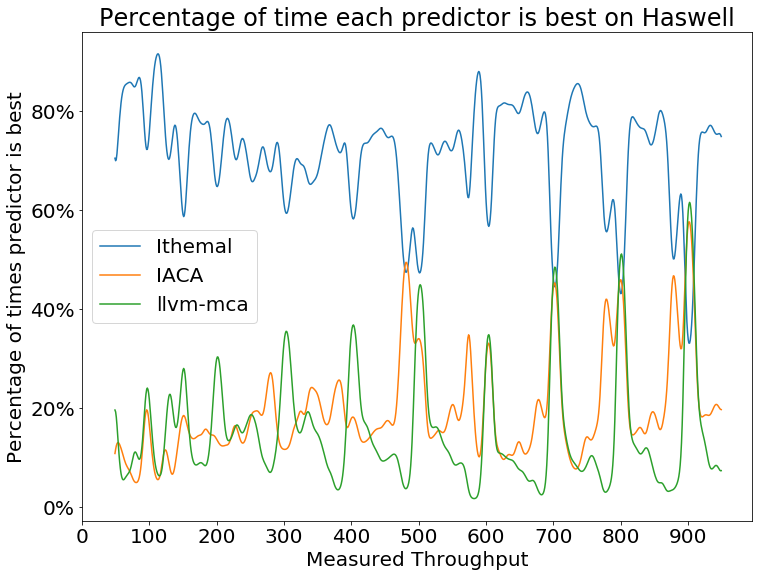
\includegraphics[width=0.33\textwidth]{figures/txput_win_haswell.png}
	}\\
	\subfloat[][Skylake - error curve]{
		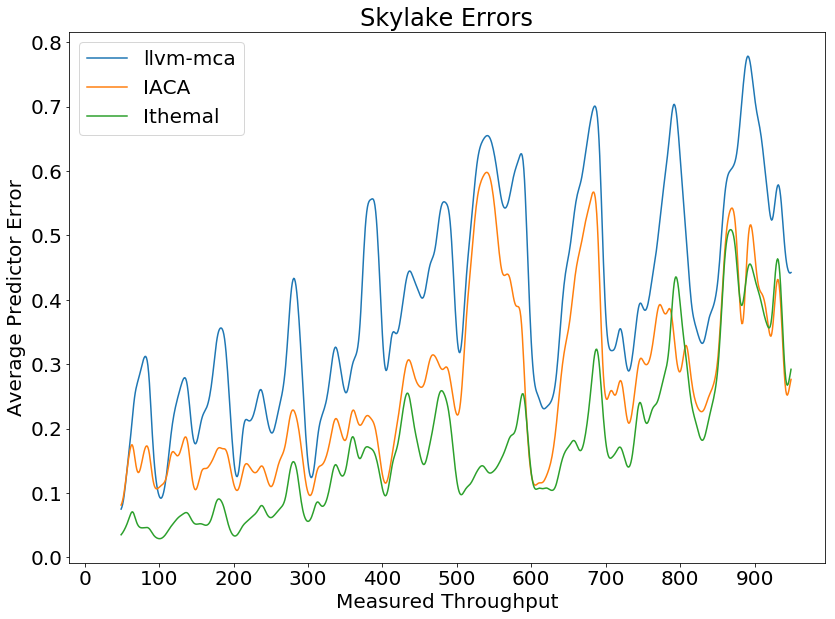
\includegraphics[width=0.33\textwidth]{figures/txput_error_skylake.png}
	}
        \subfloat[][Skylake - throughput distribution]{
		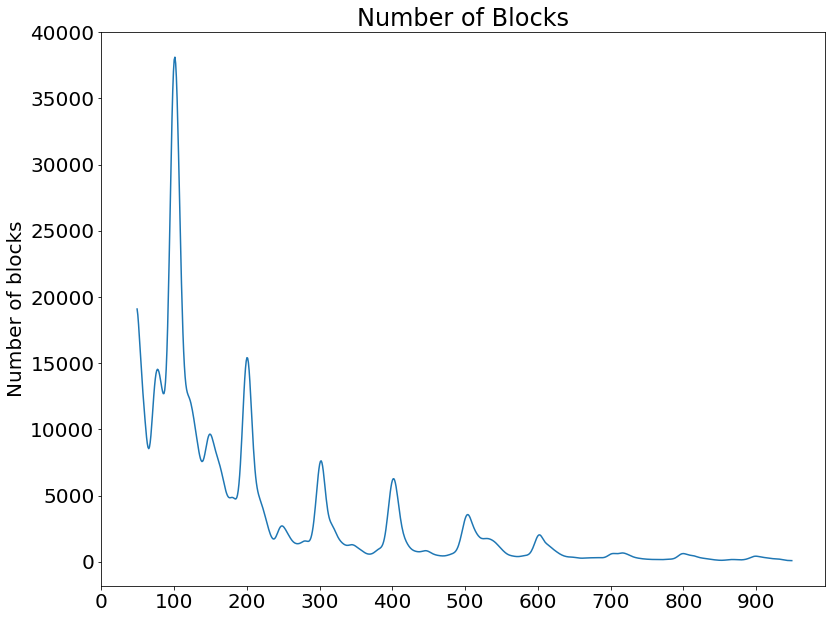
\includegraphics[width=0.33\textwidth]{figures/txput_count_skylake.png}
	}
        \subfloat[][Skylake - best predictor percentage]{
		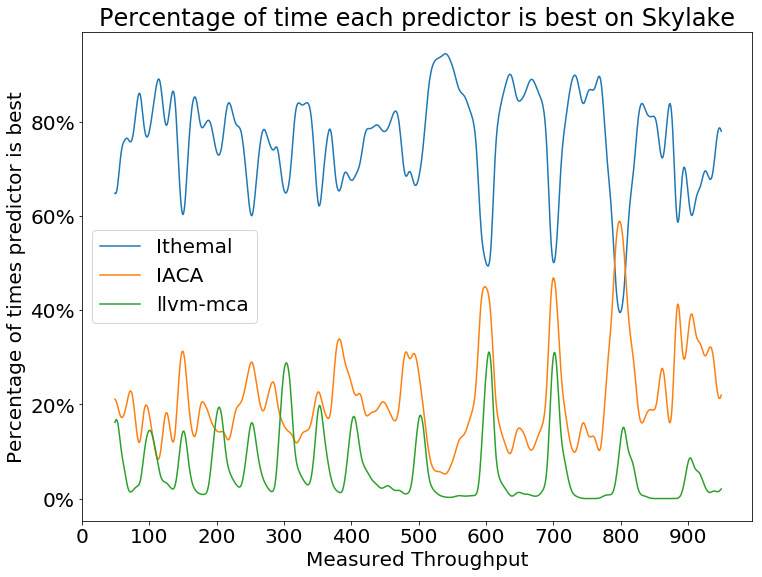
\includegraphics[width=0.33\textwidth]{figures/txput_win_skylake.png}
	}

	\caption{Average error curves and throughput distributions for different models for basic blocks with measured throughput values less than 1000 cycles under different microarchitectures for the test set}
	\label{fig:errorall}
      \end{figure*}

\section{Token RNN Architecture}
\label{app:token-rnn-architecture}

The full architecture for the Token RNN as presented in Section~\ref{sec:exploration} is shown in Figure~\ref{fig:token-rnn-architecture}.

\begin{figure*}[h!]
    \centering
    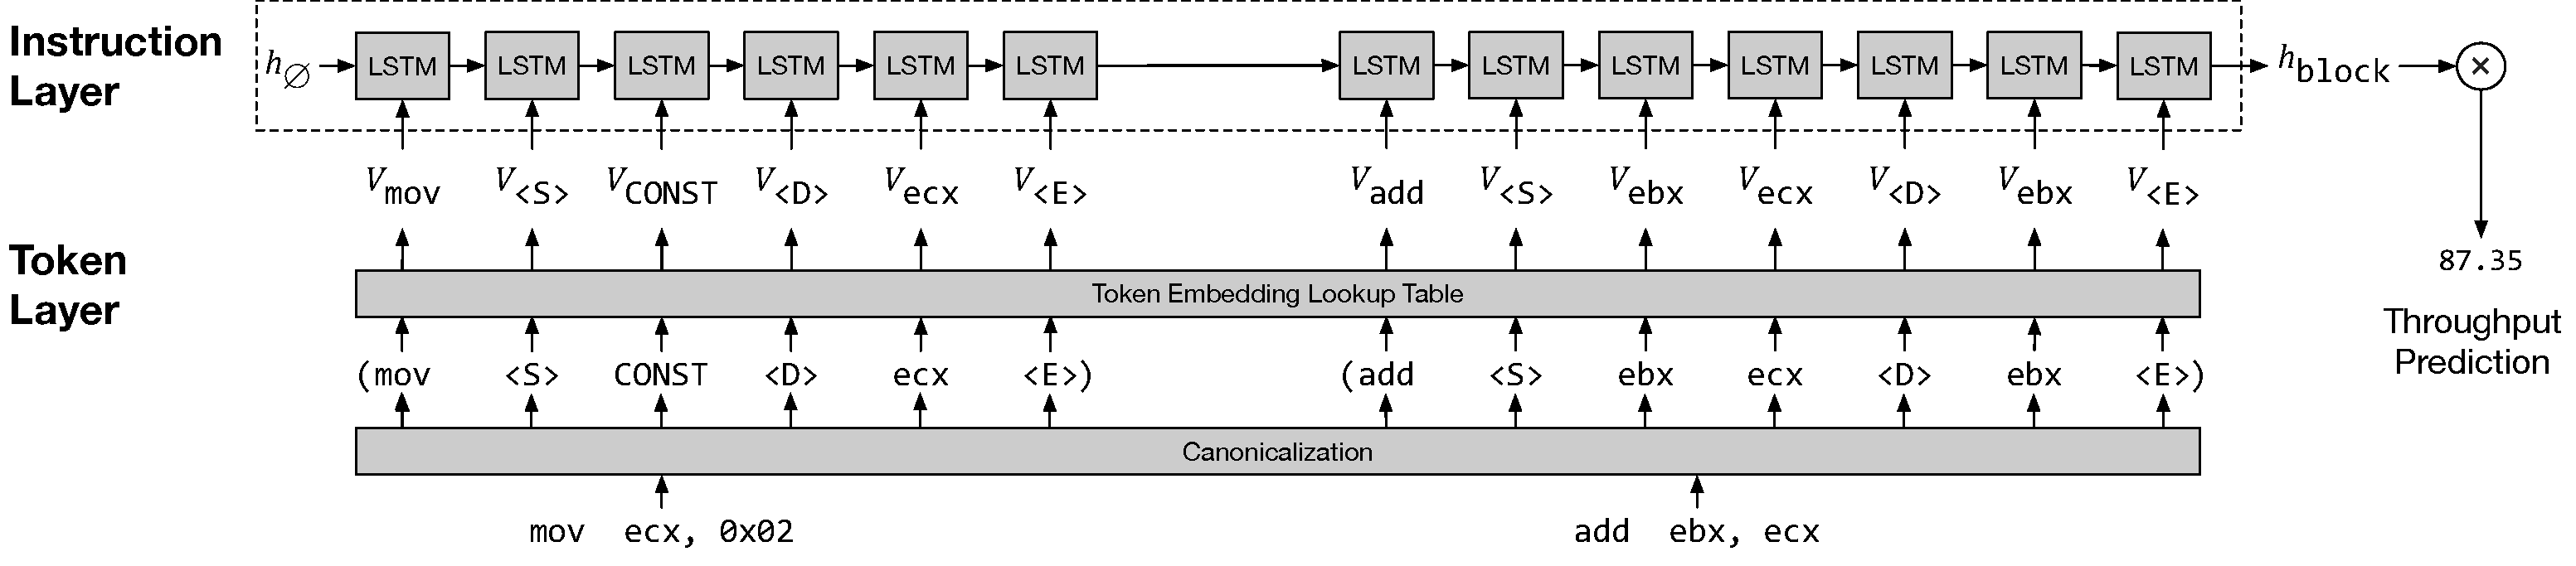
\includegraphics[width=\textwidth]{figures/diag_token_lstm.pdf}
    \vspace{-20pt}
    \caption{Token RNN Architecture}
    \label{fig:token-rnn-architecture}
\end{figure*}
